\documentclass[12pt,a4paper]{scrartcl}

%%%%%%%%%%%%%%%%%%%%%%%%%%%%%%%%%%%%%%%%%%%%%%%%%%%%%%%%%
% Validation Report                                     %
% Proof Searching and Proof checking                    %
% Computing Group Project 2010                          %
%%%%%%%%%%%%%%%%%%%%%%%%%%%%%%%%%%%%%%%%%%%%%%%%%%%%%%%%%

% standard packages
\usepackage[latin1]{inputenc}
\usepackage{amssymb, amsmath, amsthm}
\usepackage{fancyhdr}
\usepackage{graphicx}
\usepackage{longtable}

% for the code listings (if any)
\usepackage{listings}
\lstset{language=Haskell, numbers=left, 
  showstringspaces=false, frame=single}

% double spacing
\usepackage{setspace}
\doublespacing

\newcommand{\meeting}[6]{%
\begin{center}%
\begin{longtable}{| p{3.5cm} | | p{13cm} |}%
\hline%
\textbf{Date:} & #1 \\%
\hline%
\textbf{People present:} &#2 \\%
\hline%
\textbf{Points discussed:} &#3\\%
\hline%
\textbf{Achievements:} &#4 \\%
\hline%
\textbf{Agreements:} &#5 \\%
\hline%
\textbf{Tasks assigned:} &#6  \\%
\hline%
\end{longtable}%
\end{center}%
\bigbreak
}

\begin{document}

% the first page
\thispagestyle{empty}
\begin{titlepage}
  \begin{center}
    \vspace*{\fill}
            {{\Large Imperial College London\\ Department of Computing\\}}
            \vfill {{\Huge Proof Searching \& Proof Checking \\
                \vspace{0.2cm}
                     Software Validation Report}}\\
            \vfill {{\large Computing Group Project\\ 
                Supervisor: Dirk Pattinson\\ Autumn 2010}}
            \vfill {Jannis Bulian, jb1508@ic.ac.uk, 567339 \\
                    Michal Parusinski, mgp08@ic.ac.uk, 566542 \\
                    Ka Wai Cheng, kwc108@ic.ac.uk, 548464\\
                    Saguy Benaim, ssb08@ic.ac.uk, 552374}
  \end{center}
\end{titlepage}

\newpage

\tableofcontents
\thispagestyle{empty}

\newpage

\section{Summary}
In this report, we will detail the software validation methods used in the development of this project, Proof Searching and Proof Checking, and also an account of the group management and activities.

Software validation methods include the use of unit testing, HLint, code reviews, stress testing and a combination of a combination of grey-box and white-box testing.

\section{Unit Testing}
For our project, there is very little potential ethical issues. The Haskell Programming language has no license restrictions regarding written code and we are making our project open source, making it openly available for use for free. All required software which may be required for the optimal use of the system will be freely available such as Latex.

A possible ethical issue is our program may be used in the process of planning malicious activities. However, we will not be able to restrict how our written program will be used in practice since our project is simply constructs proofs/models and checks proofs/models are correct.

The environmental impacts of the system when it is deployed are limited. Supply of the developed system and required materials to develop the system are electronic and therefore have less environmental impact. The outputs of the system (messages, proofs and graphical models) will only be displayed onscreen and stored electronically.

No additional hardware to the typical computer system will be needed and hence no computing equipment will need to be replaced and wasted as a consequence of users choosing to use our system. Also, Haskell code is relatively shorter than writing the same program in other programming languages, so less storage capacity is needed for the actual program files.

On the other hand, since proof and model searching and checking could potentially take a very long time, it will be important to increase algorithmic efficiency as to improve the energy efficiency of our program. To do this, some time will be spent on optimising code and exploring possibly more efficient algorithms, however, long computation time may be unavoidable to ensure the correctness of the program.

By using Google Code, the environmental impact of the development of the system will be reduced, since comments on code and code reviews are well integrated and works just as well if not better than commenting by hand on printed code. Our main form of communication outside of meetings is via email; and reports and logs are directly managed and submitted electronically. This minimises the environmental impact as little to no paper will be used and telecommuting can be used to reduce travelling costs to the environment.

Meetings are held on campus, which will have no extra cost as they are fixed costs incurring such as heating and lighting, and when team members are all on site not only to attend these group meetings such as lectures. Hence this reduces the environmental impact of travelling. These meetings are necessary for effective face-to-face communication to discuss and explain complex algorithms or problems, which are very likely to occur in our project.

\section{General Validation}
\begin{frame}
  \frametitle{Tableaux Calculus}
  {\bf Question:} How do we formally show that there is no model?
  \pause
  \bigskip
  We use a formal proof system: The tableaux calculus. \\
  We have four rules:
  \[
  (\bot) \, \Gamma: \frac{X; A; \lnot A}{\bot}, \quad
  (\sqcap) \, \Gamma: \frac{X; C \sqcap D}{X; C; D}, \quad
  (\sqcup) \, \Gamma: \frac{X; C \sqcup D}{X; C | X; D},
  \]
  \[
  (\exists R) \, \Gamma: \frac{X; \exists R. C}{\{D | \forall R.D \in X\};  C ; \Gamma}.
  \]
  \pause
  We have a proof if we can \emph{close} all the branches with a $\bot$.
  \pause
  This proof system is sound \& complete with respect to $\mathcal{ALC}$.
\end{frame}

\begin{frame}
  \frametitle{The program: main components}
  \begin{figure}
  \begin{center}
    \includegraphics[scale=0.2]{design.jpeg}
  \end{center}
\end{figure}
\end{frame}

\begin{frame}
  \frametitle{The program: main components}
\textbf{Parser.} Automatically generated from a grammar. \\
\pause
\textbf{Proof/Model Search.} Gets a knowledgebase and a set of concepts. Generates either
a proof or model. \\
\pause
\textbf{Proof Checker.} Checks if a proof is correct. If not, gives helpful advice. \\
\pause
\textbf{Model Checker.} Checks if a model is correct. If not, gives helpful advice. \\
\end{frame}

\section{Managerial Documentation}
\subsection*{Management Tools}

We hosted our project on Google Code which offered us various development and management tools. As part of the Google Code environment, we used Mercurial Version Control and reported bugs and other issues on the Issue Tracker. We also used the Wiki and Code review options in Google which helped us to provide documentation and communicate our changes efficiently and effectively. The use of Google's environment helped us centralise all the management tools in one place which is easy to access and control.

We also used cabal, a system for building and packaging Haskell libraries and programs, to manage different packages and libraries in our project. 

\subsection*{Management Policies}

The most efficient management policy we used, was the frequent SCRUM like meetings which we held three times a week. Two meetings would be held with the groups members only. In these, we would describe the progress with respect the the set tasks, look at any problems or issues that occurred, and set new tasks for the next meeting. The other meeting would be held with our supervisor in which we discussed next iterations and any issues regarding the code. 

These meeting were key in the way code was changed. Using Mercurial we ensured code changes were coordinated. Code reviews and issues in the Issue tracker were addressed and code was changed accordingly. 

Before submitting code we run the unit tests (as a test suite) to see if any tests broke as a result of our code changes. We built additional unit tests and added them to the test suit. The tests suite was managed using cabal, which allowed an easy way of running the test suite. We also run \emph{hlint} to improve the code quality before committing the changes using Mercurial. 

\subsection*{Knowledge Transfer}

Most knowledge transfer was done through the meetings described above. In these informal meeting we discuss technical and theoretical issues
and scheduled meetings. During these meetings, we solved any problems that has risen
from a gap in our technical or theoretical knowledge. Outside of meetings, we use code
reviews through Google Code to help other group members improve their code and share
our knowledge. The most significant knowledge transfer was made during the meeting with our supervisor, were the more difficult concepts and later iterations were discussed.

\subsection*{Group Meetings and Tasks}

All group meetings, their dates and people attended are recorded in the log book. The log book itself contains detailed description of these tasks and is included in the appendix. The following table gives the distribution of tasks between group members. Additional tasks of code reviews, peer reviews and attending meetings or discussions were not included as tasks.

\week{11 October 2010 - 17 October 2010}%
{ \begin{itemize} 
    \item Investigated different possibilities for collaboration platforms,
tried out github, and set up a Google Code account, including some
initial setting (3 hours)
    \item Read papers and think about design (6 hours)
 \end{itemize} 
}%
{ \begin{itemize} 
    \item Read papers and think about design (6 hours)
 \end{itemize} 
}%
{ \begin{itemize} 
    \item Read papers and think about design (6 hours)
 \end{itemize} 
}%
{ \begin{itemize} 
    \item Read papers and think about design (6 hours)
 \end{itemize} 
}%

\week{18 October 2010 - 24 October 2010}%
{ \begin{itemize} 
    \item Set up a template for the first report and start writing own part,
proofreading and discussing other parts (4 hours)
    \item Read more papers, improved and elaborated design (5 hours)
 \end{itemize} 
}%
{ \begin{itemize} 
    \item Wrote own part of report, proofreading and discussing other parts (4 hours)
    \item Read more papers, improved and elaborated design (5 hours)
 \end{itemize} 
}%
{ \begin{itemize} 
    \item Wrote own part of report, proofreading and discussing other parts (4 hours)
    \item Read more papers, improved and elaborated design (5 hours)
 \end{itemize} 
}%
{ \begin{itemize} 
    \item Wrote own part of report, proofreading and discussing other parts (4 hours)
    \item Read more papers, improved and elaborated design (5 hours)
    \item Set up some additional software (1 hour)
 \end{itemize} 
}%

\week{25 October 2010 - 31 October 2010}%
{ \begin{itemize} 
  \item Finalise report, proofread the other
parts and rewrite the introduction  (4 hours)
 \item Read additional papers (2 hours)
 \item Start work on the proof/model searcher (4 hours)
 \end{itemize} 
}%
{ \begin{itemize} 
 \item Finalised report and proofread (4 hours)
 \item Started work on the proof/model searcher, jointly with Jannis (4 hours)
 \item Wrote unit tests for proof/model searcher (8 hours)
 \end{itemize} 
}%
{ \begin{itemize} 
  \item Finalised report and proofread (4 hours)
  \item Created Signature.hs/Proof.hs/Model.hs (4 hours)
  \item Wrote unit tests (2 hours)
 \end{itemize} 
}%
{ \begin{itemize} 
  \item Finalised report and proofread (4 hours)
  \item Wrote proof checker  (4 hours)
  \item Wrote unit tests for proof checker  (2 hours)
 \end{itemize} 
}%

\week{1 November 2010 - 7 November 2010}%
{ \begin{itemize} 
  \item Finished first implementation of proof/model searcher (6 hours)
  \item Fixed some issues with the proof/model searcher (2 hours)
  \item Wrote a main file (1 hour)
 \end{itemize} 
}%
{ \begin{itemize} 
 \item Added more unit tests for proof/model searcher (4 hours)
 \end{itemize} 
}%
{ \begin{itemize} 
  \item Added precedence rule for Description Logic (2 hours)
  \item A function sending concept to its negation normal form (1.5 hours)
  \item Model checker for atomic concepts (2 hours)
  \item Wrote tests for the above (1 hour)
 \end{itemize} 
}%
{ \begin{itemize} 
  \item Wrote proof checker  (3 hours)
  \item Wrote unit tests for proof checker  (2 hours)
  \item Tested and fixed bugs (1 hour)
 \end{itemize} 
}%

\week{8 November 2010 - 14 November 2010}%
{ \begin{itemize} 
 \item Started work on progress report, setting up a template (3 hours)
 \item Made the interfaces for proof searcher / proof checker match (1 hour)
 \item Fixed bugs in the proof/model searcher and improve style (4h)
 \item Factor out some useful functions and added several new ones to a
 dedicated utils file (2h)
 \end{itemize} 
}%
{ \begin{itemize} 
 \item Start work of progress report (3 hours)
 \item Started work on cycles within proof/model searcher (6 hours) 
 \item Added additional tests for proof/model searcher (1 hour)
 \end{itemize} 
}%
{ \begin{itemize} 
 \item Basic testing for model checker (3 hours)
 \item Model checker without reports for failure (4 hours)
 \end{itemize} 
}%
{ \begin{itemize} 
 \item Added additional checks on inputs in Proof Checker (3 hours)
 \item Added more unit tests (2 hours)
 \item Improved code and changes to code due to changes in proof tree data structure (1 hour)
 \item Testing and fixing bugs (1 hour)
 \end{itemize} 
}%

\week{15 November 2010 - 21 November 2010}%
{ \begin{itemize} 
 \item Fixed more bugs in the proof/model searcher (3 hours)
 \item Wrote a parser for modal K formulas into ACL (8 hours)
 \item Worked on improving some of the new utilities in ProofUtils (2 hours)
 \item Wrote parser for user input (2 hours)
 \end{itemize} 
}%
{ \begin{itemize} 
 \item Work on cycles within proof/model searcher (5 hours)
 \item Added additional tests for proof/model searcher to test cycles (3 hour)
 \end{itemize} 
}%
{ \begin{itemize} 
 \item Extensive testing for the model checker (2 hours)
 \item Model checker with reports for failure (3 hours)
 \item Cabal package management system setup (1 hours)
 \item Function to perform all tests (1 hour)
 \end{itemize} 
}%
{ \begin{itemize} 
 \item Improved code and messages produced by Proof Checker and adapting unit tests (1 hour)
 \item Testing and fixing bugs after changes to Proof Checker (1 hour)
 \item Wrote separate parsers for benchmark files using Happy (4 hours)
 \item Combined parsers to use reuse grammar rules, tokens, functions (2 hours)
 \item Testing parser and fixing bugs (1 hour)
 \end{itemize} 
}%

\week{22 November 2010 - 28 November 2010}%
{ \begin{itemize} 
 \item Further improved user input language (2 hours)
 \item Wrote tests for the user input language (3 hours)
 \item Fixed some of the proof search tests (1 hours)
 \item Cleaned up of the parser and improved performance (2 hours)
 \end{itemize} 
}%
{ \begin{itemize} 
 \item More tests for cycles (3 hours)
 \item Additional work on cycles implementation (7 hours)
 \end{itemize} 
}%
{ \begin{itemize} 
\item Creation of a test generating function (3 hours)
\item Improved clarity of the units tests combined them together (15 hours)
 \end{itemize} 
}%
{ \begin{itemize} 
  \item Improved parser to reuse code and remove redundant code, grammar rules, tokens (2 hours)
  \item Improve proof checker messages (1 hour)
  \item Adapted unit tests to use the clearer function written by Michal (2 hours)
  \item Add unit tests for lexical analysis of benchmark files and fixed bugs revealed (3 hours)
 \end{itemize} 
}%

\week{29 November 2010 - 5 December 2010}%
{ \begin{itemize} 
 \item Improved the test setup and including the parser tests (2 hours
 \item Fixed more bugs and factored out some code as well as further improvements in
the proof search (5 hours)
 \end{itemize} 
}%
{ \begin{itemize} 
 \item General improvements in proof search (3 hours)
 \item Additional work on cycles implementation (5 hours)
 \end{itemize} 
}%
{ \begin{itemize} 
\item Parser test for simple cases (2 hours)
\item Helped you with debugging (2 hours)
 \end{itemize} 
}%
{ \begin{itemize} 
 \item Locating the exists bug and finding the smallest case which produces the bug (5 hours)
 \end{itemize} 
}%

\week{6 November 2010 - 11 December 2010}%
{ \begin{itemize} 
  \item Helping fix problems with caching (part of proof/model searcher), studying code (3 hours)
 \item  Writing validation report, settings up templates (4 hours)
 \end{itemize} 
}%
{ \begin{itemize} 
 \item Fix problem with caching (5 hours)
 \item Wrote own part of validation report (4 hours)
 \end{itemize} 
}%
{ \begin{itemize} 
 \item Wrote own part of validation report (4 hours)
 \item Function to create pdf's containing the proof (3 hours)
 \end{itemize} 
}%
{ \begin{itemize} 
  \item Wrote own part of validation report (4 hours)
 \item Model graphical output into DOT language (5 hours)
 \item Unit tests for model output (3 hours)
 \item Testing and fixing bugs for model output (2 hours)
 \end{itemize} 
}%

\subsection{Log-Book}
The aim of our project was to create a solver for Description Logic, a
knowlegde representation language. We have managed to create a softare
intented for the GHC platform that decide satisfiability or otherwise
unsatisfiability of a given knowledge base together with some
concepts. Unlike most solvers for Description Logic the one we
create is intented for academia.



\end{document}
